% Adjust these for the path of the theme and its graphics, relative to this file
%\usepackage{beamerthemeFalmouthGamesAcademy}
\usepackage{../../beamerthemeFalmouthGamesAcademy}
\usepackage{multimedia}
\graphicspath{ {../../} }

% Default language for code listings
\lstset{language=C++,
        morekeywords={each,in,nullptr}
}

% From http://blog.virtualglobebook.com/2011/02/syntax-highlighting-c-and-glsl-source.html

\lstdefinelanguage{GLSL}
{
sensitive=true,
morekeywords=[1]{
attribute, const, uniform, varying,
layout, centroid, flat, smooth,
noperspective, break, continue, do,
for, while, switch, case, default, if,
else, in, out, inout, float, int, void,
bool, true, false, invariant, discard,
return, mat2, mat3, mat4, mat2x2, mat2x3,
mat2x4, mat3x2, mat3x3, mat3x4, mat4x2,
mat4x3, mat4x4, vec2, vec3, vec4, ivec2,
ivec3, ivec4, bvec2, bvec3, bvec4, uint,
uvec2, uvec3, uvec4, lowp, mediump, highp,
precision, sampler1D, sampler2D, sampler3D,
samplerCube, sampler1DShadow,
sampler2DShadow, samplerCubeShadow,
sampler1DArray, sampler2DArray,
sampler1DArrayShadow, sampler2DArrayShadow,
isampler1D, isampler2D, isampler3D,
isamplerCube, isampler1DArray,
isampler2DArray, usampler1D, usampler2D,
usampler3D, usamplerCube, usampler1DArray,
usampler2DArray, sampler2DRect,
sampler2DRectShadow, isampler2DRect,
usampler2DRect, samplerBuffer,
isamplerBuffer, usamplerBuffer, sampler2DMS,
isampler2DMS, usampler2DMS,
sampler2DMSArray, isampler2DMSArray,
usampler2DMSArray, struct},
morekeywords=[2]{
radians,degrees,sin,cos,tan,asin,acos,atan,
atan,sinh,cosh,tanh,asinh,acosh,atanh,pow,
exp,log,exp2,log2,sqrt,inversesqrt,abs,sign,
floor,trunc,round,roundEven,ceil,fract,mod,modf,
min,max,clamp,mix,step,smoothstep,isnan,isinf,
floatBitsToInt,floatBitsToUint,intBitsToFloat,
uintBitsToFloat,length,distance,dot,cross,
normalize,faceforward,reflect,refract,
matrixCompMult,outerProduct,transpose,
determinant,inverse,lessThan,lessThanEqual,
greaterThan,greaterThanEqual,equal,notEqual,
any,all,not,textureSize,texture,textureProj,
textureLod,textureOffset,texelFetch,
texelFetchOffset,textureProjOffset,
textureLodOffset,textureProjLod,
textureProjLodOffset,textureGrad,
textureGradOffset,textureProjGrad,
textureProjGradOffset,texture1D,texture1DProj,
texture1DProjLod,texture2D,texture2DProj,
texture2DLod,texture2DProjLod,texture3D,
texture3DProj,texture3DLod,texture3DProjLod,
textureCube,textureCubeLod,shadow1D,shadow2D,
shadow1DProj,shadow2DProj,shadow1DLod,
shadow2DLod,shadow1DProjLod,shadow2DProjLod,
dFdx,dFdy,fwidth,noise1,noise2,noise3,noise4,
EmitVertex,EndPrimitive},
morekeywords=[3]{
gl_VertexID,gl_InstanceID,gl_Position,
gl_PointSize,gl_ClipDistance,gl_PerVertex,
gl_Layer,gl_ClipVertex,gl_FragCoord,
gl_FrontFacing,gl_ClipDistance,gl_FragColor,
gl_FragData,gl_MaxDrawBuffers,gl_FragDepth,
gl_PointCoord,gl_PrimitiveID,
gl_MaxVertexAttribs,gl_MaxVertexUniformComponents,
gl_MaxVaryingFloats,gl_MaxVaryingComponents,
gl_MaxVertexOutputComponents,
gl_MaxGeometryInputComponents,
gl_MaxGeometryOutputComponents,
gl_MaxFragmentInputComponents,
gl_MaxVertexTextureImageUnits,
gl_MaxCombinedTextureImageUnits,
gl_MaxTextureImageUnits,
gl_MaxFragmentUniformComponents,
gl_MaxDrawBuffers,gl_MaxClipDistances,
gl_MaxGeometryTextureImageUnits,
gl_MaxGeometryOutputVertices,
gl_MaxGeometryOutputVertices,
gl_MaxGeometryTotalOutputComponents,
gl_MaxGeometryUniformComponents,
gl_MaxGeometryVaryingComponents,gl_DepthRange},
morecomment=[l]{//},
morecomment=[s]{/*}{*/},
morecomment=[l][keywordstyle4]{\#},
}


% For strikethrough effect
\usepackage[normalem]{ulem}
\usepackage{wasysym}

\usepackage{pdfpages}

% http://www.texample.net/tikz/examples/state-machine/
\usetikzlibrary{arrows,automata}

\newcommand{\modulecode}{COMP260}\newcommand{\moduletitle}{Distributed Systems}\newcommand{\sessionnumber}{5}

\begin{document}
\title{\sessionnumber: Vertices, Transforms \& Projections}
\subtitle{\modulecode: \moduletitle}

\frame{\titlepage} 

\begin{frame}{Learning outcomes}
	By the end of this week, you should be able to:
	\begin{itemize}
		\item \textbf{Recall} alternative ways to represent mesh vertices in memory.
		\item \textbf{Apply} basic transforms using the GLM library.
		\item \textbf{Explain} the constituents of the model-view-projection matrix and how it can be used to create a first-person camera controller.
	\end{itemize}
\end{frame}

\begin{frame}{Agenda}
	\begin{itemize}
		\pause\item Lecture (async):
		\begin{itemize}
			\item \textbf{Compare} different ways to store vertex data in memory.
			\item \textbf{Review} the transforms required to display 3D objects on a 2D screen.
		\end{itemize}
		\pause\item Workshop (sync):
		\begin{itemize}
			\item \textbf{Adapt} our basic triangle implementation to draw meshes with multiple triangles efficiently.
			\item \textbf{Experiment} with creating transforms using GLM and using them to move objects and the camera.
		\end{itemize}
	\end{itemize}
\end{frame}

\begin{frame}{Schedule}
	\begin{center}
		\begin{tabular}{|c c|}
			\hline
			16:00-16:05 & Arrival \& sign-in \\
			\hline
			16:05-16:10 & Introduction \\
			\hline
			16:10-16:20 & Setting up (LS) \\
			\hline
			16:20-16:40 & Demo: Creating a Triangle \\
			16:40-17:00 & Exercise: Creating a Triangle (LS) \\
			\hline
			17:00-17:20 & Introduction to GLSL \\
			\hline
			17:20-17:40 & Demo: Creating Shaders \\
			17:40-18:00 & Exercise: Creating Shaders (LS) \\
			\hline
		\end{tabular}
	\end{center}
\end{frame}

\part{Element Buffer}
\frame{\partpage}

\begin{frame}{Element Buffer}
	\begin{itemize}
		\pause\item If we look at the cube sample, we are sending 36 vertices
		\pause\item This is a bit wasteful considering that some of these vertices are duplicates
		\pause\item We can use an \textbf{Element Buffer} to optimise our drawing
		\pause\item An Element Buffer holds an integer which is an offset into a Vertex Buffer
	\end{itemize}
\end{frame}

\begin{frame}{Creating \& Using Element Buffer}
	\begin{center}
		Live Coding
	\end{center}
\end{frame}

\begin{frame}{Exercise 1 - Let's draw a square!}
\begin{center}
	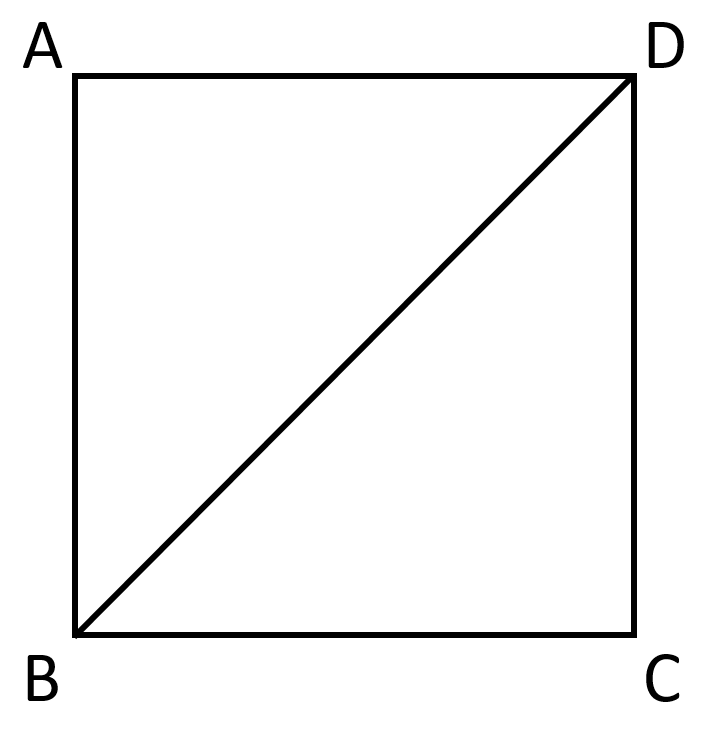
\includegraphics[height=0.8\textheight]{square_vertices}
\end{center}
\end{frame}

\begin{frame}{Exercise 2 - Let's draw a cube!}
	\begin{center}
	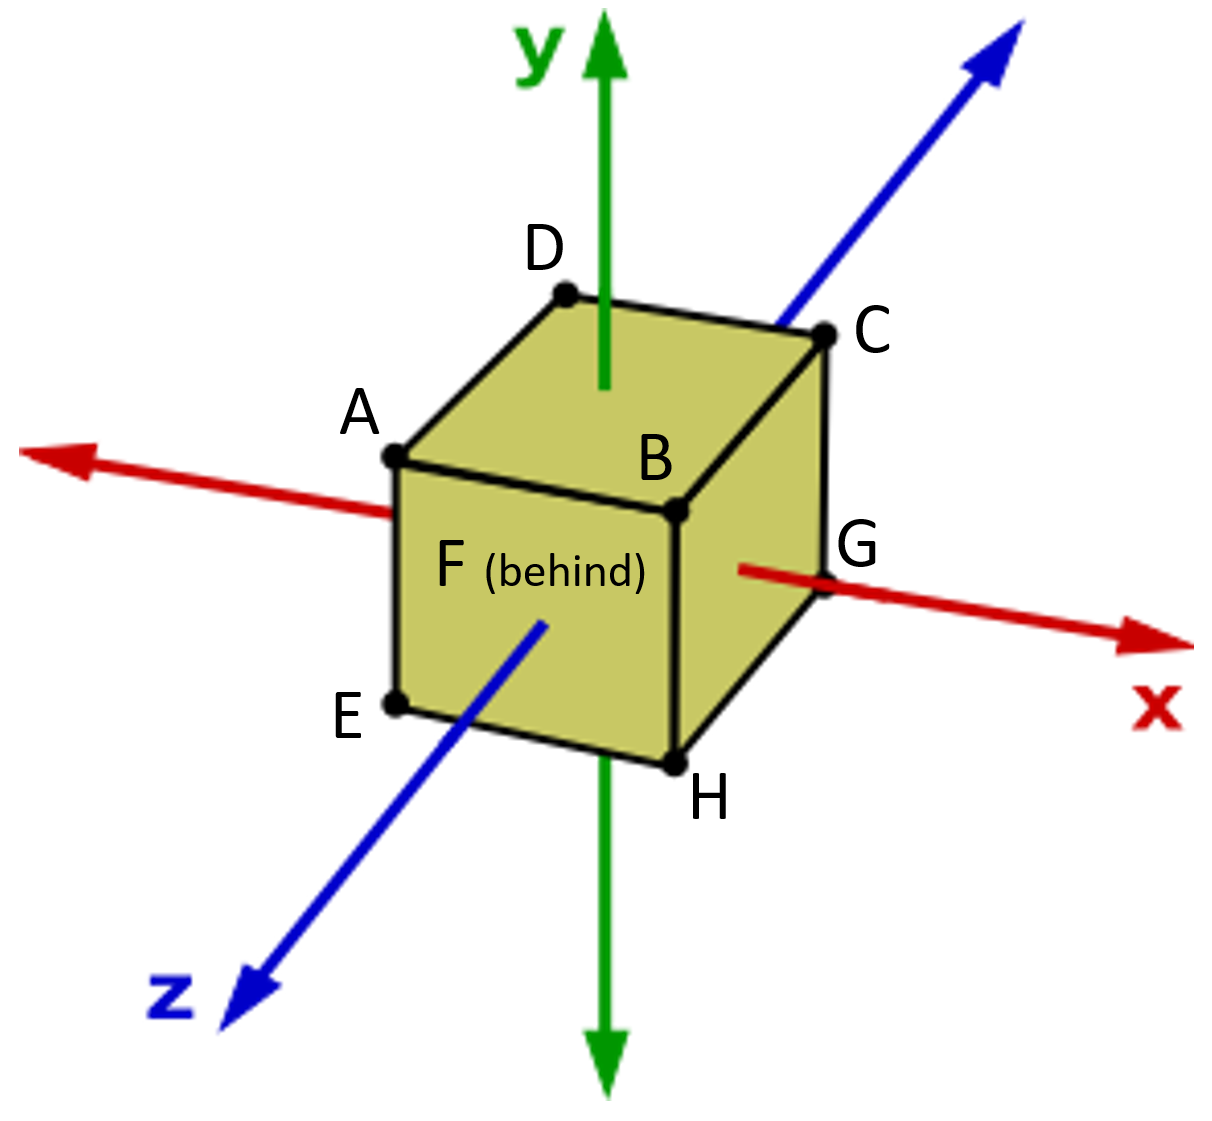
\includegraphics[height=0.8\textheight]{cube_vertices}
	\end{center}
\end{frame}

\begin{frame}{Exercise 3 - Element Buffer}
	\begin{itemize}
		\item Create a cube using an Element Buffer
		\item Create a function which fills a Vertex Buffer and Element Buffer for drawing a Sphere
	\end{itemize}
\end{frame}

\begin{frame}{Further Reading - Interleaved Vertices}
	\begin{itemize}
		\item iOS Development Docs - \url{https://developer.apple.com/library/content/documentation/3DDrawing/Conceptual/OpenGLES_ProgrammingGuide/TechniquesforWorkingwithVertexData/TechniquesforWorkingwithVertexData.html}
		\item To interleave or not to interleave - \url{https://anteru.net/blog/2016/02/14/3119/index.html}
		\item Vertex Specification Best Practices - \url{https://www.khronos.org/opengl/wiki/Vertex_Specification_Best_Practices}
	\end{itemize}
\end{frame}

\begin{frame}{Further Reading - Element Buffer}
	\begin{itemize}
		\item VBO indexing - \url{http://www.opengl-tutorial.org/intermediate-tutorials/tutorial-9-vbo-indexing/}
		\item Element Buffer - \url{https://goharsha.com/lwjgl-tutorial-series/element-buffer-objects/}
	\end{itemize}
\end{frame}



\part{Transformations in GLM}
\frame{\partpage}

\begin{frame}{Right hand rule}
	\pause OpenGL uses a \textbf{right-handed coordinate system}
	\pause \begin{center}
		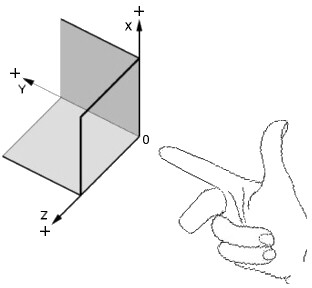
\includegraphics[width=0.3\textwidth]{RightHandRule}
	\end{center}
	\begin{itemize}
		\pause\item The \textbf{$x$-axis} points towards the \textbf{right-hand side} of the screen
		\pause\item The \textbf{$y$-axis} points towards the \textbf{top} of the screen
		\pause\item The \textbf{$z$-axis} points \textbf{out} of the screen
	\end{itemize}
\end{frame}

\begin{frame}{Transformations and matrices}
	\begin{itemize}
		\pause\item A \textbf{transformation} is a \textbf{mathematical function} that \textbf{changes points in space}
		\pause\item E.g.\ shifts them, rotates them, scales them, ...
		\pause\item Many useful transformations can be \textbf{represented} by matrices
		\pause\item Multiplying these matrices together \textbf{combines} the transformations
		\pause\item Multiplying a vector by the matrix \textbf{applies} the transformation
	\end{itemize}
\end{frame}

\begin{frame}[fragile]{GLM}
	\begin{itemize}
		\pause\item We will use the \textbf{GLM} library to do matrix calculations for us
		\pause\item \url{http://glm.g-truc.net/}
		\pause\item GLM aims to mirror GLSL data types (\lstinline{vec4}, \lstinline{mat4} etc) in C++
		\pause\item Lets us perform calculations with vectors and matrices in C++
		\pause\item GLM types can be passed into shaders as uniforms, e.g.
			\begin{lstlisting}
// transformLocation points to a uniform of type mat4
glm::mat4 transform = ...;
glUniformMatrix4fv(transformLocation, 1, GL_FALSE,
				glm::value_ptr(transform));
			\end{lstlisting}
	\end{itemize}
\end{frame}

\begin{frame}[fragile]{Identity}
	\pause The identity transformation does not change anything
	\pause \begin{lstlisting}
// Default constructor for glm::mat4
// creates an identity matrix
glm::mat4 transform;
	\end{lstlisting}
\end{frame}

\begin{frame}[fragile]{Translation}
	\pause Translation shifts all points by the same vector offset
	\pause \begin{lstlisting}
transform = glm::translate(transform,
					glm::vec3(0.3f, 0.5f, 0.0f));
	\end{lstlisting}
\end{frame}

\begin{frame}[fragile]{Scaling}
	\pause Scaling moves all points closer or further from the origin by the same factor
	\pause \begin{lstlisting}
transform = glm::scale(transform,
				glm::vec3(1.2f, 0.5f, 1.0f));
	\end{lstlisting}
\end{frame}

\begin{frame}[fragile]{Rotation}
	\begin{itemize}
		\pause\item How do we represent a rotation in 3 dimensions?
		\pause\item One way is by specifying the \textbf{axis} (as a vector) and the \textbf{angle} (in radians)
		\pause\item Axis always runs through the origin
	\end{itemize}
	\pause \begin{lstlisting}
float angle = glm::pi<float>() * 0.5f;
glm::vec3 axis(0, 0, 1);
transform = glm::rotate(transform, angle, axis);
	\end{lstlisting}
\end{frame}

\begin{frame}[fragile]{Combining transformations}
	\pause \begin{lstlisting}
transform = glm::translate(transform,
					glm::vec3(0.5f, 0.5f, 0.0f));
transform = glm::rotate(transform, angle, axis);
	\end{lstlisting}
	\begin{itemize}
		\pause\item Transformations \textbf{do not commute} in general ---
			changing the order will change the result
		\pause\item The order they are applied is the \textbf{reverse} of what you might think ---
			i.e.\ the above rotates \textbf{then} translates
	\end{itemize}
\end{frame}
\part{First person camera control}
\frame{\partpage}

\begin{frame}{The plan}
	\begin{itemize}
		\pause\item Represent the player's \textbf{position} by a 3D vector
		\pause\item Represent the player's \textbf{orientation} by Euler angles
		\pause\item Mouse events change these angles
		\pause\item View matrix is calculated using position and orientation
		\pause\item To move forwards, use the Euler angles to find the ``forward'' vector,
			and offset the position by this vector
	\end{itemize}
\end{frame}

\begin{frame}{Keyboard and mouse in SDL}
	\pause Use \textbf{relative mouse mode}
	\begin{itemize}
		\pause\item Hides the mouse pointer
		\pause\item Prevents the mouse pointer from hitting the edge of the screen
		\pause\item Gives us the distance the mouse has moved since last frame, rather than its current position
	\end{itemize}
	\pause Use \lstinline{SDL_GetKeyboardState} instead of handling individual keyboard events
	\begin{itemize}
		\pause\item Allows us to check on every frame whether the key is held down
		\pause\item Otherwise, the player will move jerkily according to the key repeat rate
	\end{itemize}
\end{frame}



\end{document}
